% Kompiuterijos katedros šablonas
% Template of Department of Computer Science II
% Versija 1.0 2015 m. kovas [ March, 2015]


\documentclass[a4paper,12pt,fleqn]{article}
\usepackage[unicode,colorlinks=false]{hyperref}


\usepackage[utf8x]{inputenc}
%

\usepackage[L7x]{fontenc}
\usepackage{times}
\usepackage{ucs}
\usepackage{microtype}
\DisableLigatures{encoding = *, family = *}
% \DisableLigatures[f]{encoding = *, family


 %package to switch the language
\usepackage{etoolbox}

  %set up of the page margins
\usepackage[top=2cm, bottom=2cm, left=3cm, right=1.5cm]{geometry}

 %1.1 line spacing
\linespread{1.1}


  %page numbering at the right side
\usepackage{fancyhdr}
\pagestyle{fancyplain}
\fancyhf{}
\renewcommand{\headrulewidth}{0pt} 
\fancyhfoffset[RO]{0cm}

  %to number at the bottom (exchange lines to number at the top)
\rfoot{\thepage}
  %\rhead{\thepage} %

% \usepackage[usenames,dvipsnames]{pstricks}
\urlstyle{same}
\hypersetup{
%  citecolor=Blue,
%  linkcolor=Blue,
%  urlcolor=Blue
pdfborder={0 0 0 }
}

 %for includegraphics
\usepackage{graphicx}



\usepackage[toc,page]{appendix}


\usepackage{caption}

 %for source codes
\usepackage{listings}
\lstset{commentstyle=\color{red},xleftmargin=10pt, framexleftmargin=6pt, numbersep=1mm, frame=single, numbers=left,numberstyle=\footnotesize,extendedchars=\true, inputencoding=utf8x,basicstyle=\footnotesize,extendedchars=true,
 keywordstyle=\color{black}\bfseries, breaklines=true, breakautoindent=true,framesep=8pt,linewidth=0.95\textwidth
}

 %for algorithms
\usepackage{algorithm}
\usepackage{algorithmic}
 %instead of the above two packages we can use algorithms2e
 %\usepackage[boxed,linesnumbered,vlined,slide]{algorithm2e}

 %special symbols
\usepackage{amsfonts}
\usepackage{amssymb}
\usepackage{amsmath}

 %for theorem like environments
\usepackage{amsthm}

 \usepackage{datetime}
 \renewcommand{\dateseparator}{--}


% SI system units
\usepackage{siunitx}
\sisetup{detect-all}
% Problem with fonts \SI{x.xx}{\micro\metre}, solved with updmap-sys --enable Map=utm.map
\renewcommand{\sfdefault}{uhv}
\renewcommand{\rmdefault}{utm}
\renewcommand{\ttdefault}{ucr}

% List management (itemize, etc.)
\usepackage{enumitem}

\newcommand*{\urlw}[1]{\href{#1}%
            {\nolinkurl{#1}}}

\numberwithin{equation}{section}

%%%%%%%%%%% lino įdėta
%
\usepackage{pifont,mdframed}

\newenvironment{warning}
  {\par\begin{mdframed}[linewidth=2pt,linecolor=red]%
    \begin{list}{}{\leftmargin=1cm
                   \labelwidth=\leftmargin}\item[\Large\ding{43}]}
  {\end{list}\end{mdframed}\par}
  


\newtoggle{inLithuanian}
 %If the report is in Lithuanian, it is set to true; otherwise, change to false
\settoggle{inLithuanian}{false}

%create file preface.tex for the preface text
%if preface is needed set to true
\newtoggle{needPreface}
\settoggle{needPreface}{false}

\newtoggle{signaturesOnTitlePage}
\settoggle{signaturesOnTitlePage}{false}



\theoremstyle{definition}
\newtheorem{definition}{\keyWordDefinition}
\newtheorem{example}{\keyWordExample}
\def\QED{\unskip\nobreak\hfill\kern5pt$\Box$}

\iftoggle{inLithuanian}{
%\usepackage[L7x]{fontenc}
\usepackage[english,lithuanian]{babel}

\newcommand{\todayiso}{\the\year \dateseparator \twodigit\month \dateseparator \twodigit\day}


\renewcommand{\today}{\number\year\space m. \space \ifcase\month\or
  sausio\or vasario\or kovo\or balandžio\or gegužės\or birželio\or
  liepos\or rugpjūčio\or rugsėjo\or spalio\or lapkričio\or
  gruodžio\fi
  \space\number\day\space d.}


 \usepackage{tocloft}
 \renewcommand\cftsecaftersnum{.} 
 \renewcommand\cftsubsecaftersnum{.} 
 \renewcommand\cftsubsubsecaftersnum{.}

 \usepackage{VUMIFKK}

 \DeclareCaptionLabelFormat{captionlt}{#2 #1}
   %smth is not fine with algorithms 
 \DeclareCaptionLabelFormat{captionltalg}{#2 #1 algoritmas}

 \usepackage{indentfirst}
 \renewcommand{\appendixtocname}{Priedai}
 \renewcommand{\appendixpagename}{Priedai}
 \renewcommand{\contentsname}{Turinys} 

 \renewcommand{\lstlistingname}{išeities kodas}
 \renewcommand{\figurename}{pav}
 \renewcommand{\tablename}{lentelė}


 \captionsetup*[lstlisting]{   
 labelsep=period,labelformat=captionlt
 }
 \captionsetup*[figure]{   
% labelsep=period,
 labelsep=space, %babel redefines pav to pav.
 labelformat=captionlt
 }
 \captionsetup*[table]{   
  labelsep=period,
  labelformat=captionlt
 }
 \renewcommand{\algorithmicrequire}{\textbf{Įvestis:}}
 \renewcommand{\algorithmicensure}{\textbf{Išvestis:}}

 \captionsetup*[algorithm]{   
 labelsep=period,labelformat=captionltalg
 }

\renewcommand{\thmhead}[3]{#2 #1#3}

}
{
%\usepackage[OT1,T1]{fontenc}
%\usepackage[L7x]{fontenc}

\usepackage[english]{babel}
\newcommand{\todayiso}{\twodigit\month \dateseparator \twodigit\day \dateseparator \the\year}
 \captionsetup*[algorithm]{   
 labelsep=period
 }
\captionsetup*[lstlisting]{   
 labelsep=period
 }
 \captionsetup*[figure]{   
 labelsep=period
 }
 \captionsetup*[table]{   
 labelsep=period
 }


}

%some kywords
 \def\keywordAbstract{\iftoggle{inLithuanian}{Summary}{Abstract}}
 \def\keywordAbstractOther{\iftoggle{inLithuanian}{Summary}{Summary}}
 \def\keyWordIntroduction{\iftoggle{inLithuanian}{Įvadas}{Introduction}}
 \def\keyWordConclusions{\iftoggle{inLithuanian}{Išvados ir rekomendacijos}{Conclusions and Recommendations}}

 \def\keyWordPreface{\iftoggle{inLithuanian}{Pratarmė}{Preface}}
 \def\keyWordAppendice{\iftoggle{inLithuanian}{Priedas}{Appendix}}
 \def\keyWordSignature{\iftoggle{inLithuanian}{parašas}{signature}}
 \def\keyWordDefinition{\iftoggle{inLithuanian}{apibrėžimas}{Definition}}
 \def\keyWordExample{\iftoggle{inLithuanian}{pavyzdys}{Example}}

\newcommand{\bothabstracts}[3]{
\setcounter{secnumdepth}{0}
\newpage
\hspace{2cm}
{\centering{\section{\keywordAbstract}}}

#1
\newpage
\hspace{2cm}
{\centering \section{\keywordAbstractOther}}

\begin{center}{\textbf{#2} }\end{center}

 #3
\setcounter{secnumdepth}{3}
}

 %non-numbered sections: #1 param: for labeling sec:#1, #2 -section title
\newcommand{\sectionWithoutNumber}[2]{\newpage
%\hspace{2cm}
\section*{#1}
\label{sec:#2}
\addcontentsline{toc}{section}{\nameref{sec:#2}}%{#3}
 }



\newcommand{\referenceSources}[1]{
\newpage
\cleardoublepage
\phantomsection
\iftoggle{inLithuanian}{
 \renewcommand{\refname}{Literatūros šaltiniai}

 \addcontentsline{toc}{section}{Literatūros šaltiniai}
 \markboth{\refname}{Literatūros šaltiniai}
 }
{

\addcontentsline{toc}{section}{References}
\markboth{References}{References}
}

\bibliographystyle{plain}
\bibliography{#1}
}



 \newcommand\authorsignature[1]{
\begin{flushright}
 \begin{minipage}[b]{0.45\textwidth}
  \centering
  \rule{\textwidth}{0.5pt}\\
   #1
  \end{minipage}
\end{flushright}
 }




 \newcommand\authorsignatures[5]{%
   \vspace{1cm}
   \authorsignature{#1}
   \ifstrequal{#2}{}{}{\vspace{0.3cm}
     \authorsignature{#2}
     \ifstrequal{#3}{}{}{\vspace{0.3cm}
      \authorsignature{#3}
      \ifstrequal{#4}{}{}{\vspace{0.3cm}
        \authorsignature{#4}
        \ifstrequal{#5}{}{}{\vspace{0.3cm}
         \authorsignature{#5}       
        }
      }
    }
} 
}

\newcommand{\authortitle}{
\iftoggle{signaturesOnTitlePage}{
\tiny{\keyWordSignature}
}{}
}

\newcommand{\depttitlepage}[8]
{
\thispagestyle{empty}
\begin{center}


\includegraphics[width=2cm]{jb_VU_zenklas}

%\vspace{-1cm}

\iftoggle{inLithuanian}
{ 
  VILNIAUS UNIVERSITETAS\\
  MATEMATIKOS IR INFORMATIKOS FAKULTETAS\\
  KOMPIUTERIJOS KATEDRA
}
{
  VILNIUS UNIVERSITY \\
  FACULTY OF MATHEMATICS AND INFORMATICS \\
  DEPARTMENT OF COMPUTER SCIENCE II
}

\vspace{5cm}

#1\\
\vspace{0.5cm}
\textbf{\Large #2}
\end{center}

\vspace{5cm}


\hspace{0.5\textwidth}
\begin{minipage}{0.4\textwidth}
 \begin{flushleft} 
\iftoggle{inLithuanian}
{
 \ifstrequal{#3}{}{}{Atliko:\\[5pt]}
}
{
\ifstrequal{#3}{}{}{Done by:\\[5pt]}
}

%\noindent
\begin{tabular}{@{}lr}%\setlength\tabcolsep{0pt}
\ifstrequal{#3}{}{}{#3&\hspace{2cm}\authortitle\\[5pt]}
\ifstrequal{#4}{}{}{#4&\authortitle\\[5pt]}
\ifstrequal{#5}{}{}{#5&\authortitle\\[5pt]}
\ifstrequal{#6}{}{}{#6&\authortitle\\[5pt]}
\ifstrequal{#7}{}{}{#7&\authortitle\\}
\end{tabular}

\end{flushleft}

\end{minipage}

\vspace{0.5cm}
\hspace{0.5\textwidth}
\begin{minipage}{0.4\textwidth}
 \begin{flushleft} 

\ifstrequal{#8}{}{}
{

\iftoggle{inLithuanian}
{
Vadovas:
}
{
Supervisor:
}

#8

}

\end{flushleft}

\end{minipage}


\vfill

\begin{center}
Vilnius\\
\the\year
\end{center}

\iftoggle{needPreface}{
 \sectionWithoutNumber{\keyWordPreface}{preface}
Pratarmės (Preface) informacija


\iftoggle{inLithuanian}
{
\vspace{\baselineskip}\hfill
\today
}
{
 \vspace{\baselineskip}\hfill \today
}

 \vspace{5cm}

\iftoggle{signaturesOnTitlePage}{}
{
\authorsignatures{#3}{#4}{#5}{#6}{#7}
}
}{}
\newpage
}


\begin{document}
 % #1 -report type, #2 - title, #3-7 students, #8 - supervisor
 \depttitlepage{Semester project}{Modelling of roads and road interchanges}{Caillard Mathias} 
 {}{}{}{}% students 2-5
 {dr. Krasauskas Rimvydas}

\tableofcontents


%keywords and notations if needed
\sectionWithoutNumber{Conventional glossary of terms}{keywords}{
\textbf{Road} : a couple of elements. The first element is an n-uple of straight lines, and the second one a n-uple of curves, such that every ending point of a straight line is connected to the starting point of another straight line through a curvature.
\newline
\newline
\textbf{Sampled road} : a sequence of points on a two-dimensional plane that comes from a sample process of a road.
\newline
\newline
\textbf{point} : a couple of two elements (x,y).
\newline
\newline
\textbf{curvature of a circle} : the inverse of the radiius of the circle.
\newline
\newline
\textbf{r-value} : a number between -1 and 1 that caracterize the correlation between the regression line and the dotted data.
\newline
\newline
\textbf{tangents} : a straight line that touches a curve locally at only one point, without intersection it. 
\newline
\newline
\textbf{circle of turn} : "circle of turn" Any circle that has an arc of itself included into the considered road. In other words, a "circle of turn" is an object used to display a curvature of the road.
}

%both abstracts
\bothabstracts{ During this coursework, I defined and simplified the concept of roads, which allows me to build two differents process of how to generate them graphically. Roads can be generated with minimal information : in the first approach, I used only circles in input to generate turns and straight lines. In the second approach, I used angles and distances. The main motivation was trying to understand how one can retro-engineer roads based on road dataset consisting of ordered points on a plane. My attempt of the retro-engineering process allows the user to detect straight lines of a sampled road dataset.}%tex-file of abstract in original language
{Modelling of roads and road interchanges} %if work is in LT this title should be in English
{
During this coursework, a lot of attention was provided to the creation of roads based on given inputs. Such a model requires to simplify reality. Thus, during my project, I made some simplification, definition, and hypothesis. My first definition of road is the following : A road is a couple of elements. The first element is an n-uple of straight lines, and the second one a n-uple of curves, such that every ending point of a straight line is connected to the starting point of another straight line through a curvature. This definition is close to how real roads are build : a sequence of straight lines and curves. My definition evolved through my work, and I’ll explain it bit by bit.
\newline
\newline
A deeper purpose of being able to model roads is to be capable to generate roads based on a road map dataset. To do so, it is necessary to find a way create an approximation of the real roads expressed through the dataset with “simplified roads” . This is the reverse-engineering part of my work : trying to understand what the real road interchange looks like only by using the road map dataset. That is the other main goal of this coursework.
\newline
\newline
This project involves programming, geometry and algebra, which are subjects that I’m particularly interested in. I decided during this semester homework to use Python as the programming language. Roads were generated visually by using a collection of “pyplot  functions” from the library matplotlib [4]. To a lesser extent, the  "math", "numpy", and "scipy" libraries have been used. During this project, I was able to generate roads as sequences of straight lines and portion of arc of circles. Then, I created two different algorithms for that : the first one has for input coordinates of circles of curvatures, their radiuses, and additional necessary residual information (I will explain this later). The second one generates arcs of circle with a constant radius, and has for input a starting point, lengths of lines, a radius, and angles for the curvatures. Then, I coded an attempt of reverse-engineering process: Using linear regression to detect straight line of the road. Within the scope of the coursework, I deem the modelling problem solved, but the reverse-engineering problem is not enough conclusive and incomplete.}%tex-file of abstract in other language


 %Introduction section: label is sec:intro
\sectionWithoutNumber{\keyWordIntroduction}{intro}

	A road interchange is a road junction that allows the interchange of traffic between multiple roadways. Roads interchanges use grades separation, which permits the vehicles to move through the junction fluidly, without interrupting the flow of the traffic stream, which may reduces the number of road accidents.
Grade-separated road junctions generally need a lots of space, are complicated and costly. That’s why optimization of the used space is financially interesting. Also, road interchanges are build contextually in already existing areas where space is limited. Thus, civil engineers have to find efficient ways to manage complex interchanges of traffic lines while respecting the unique spatial constraints.
\newline
Apart from the purpose of interconnecting roadways, road interchanges are also playing a role of speed regulation by imposing curves : the tighter the curvature, the slower the speed. Moreover, due to the eventual difference of height of surface transport axes, a road interchange can allows animal to cross roadways and highways more safely, which might diminish the number of accidents.
This way, stakes of road interchanges are numerous, such that patents on road interchanges had been filled. In particular, an intersection called “PINAVIA” have been created by an engineer called “Stanislaus Buteliauskas” in 2004 and patented in 2008 [1]. This road junction is designed for high-intensity roads, for the main purpose of reducing traffic congestion, increasing junction capacities, and indirectly reducing environmental pollution [1]. This new class of road junction is patented as an innovation, but it’s difficult to figure out if such a type of road interchange has been built elsewhere in the world. The inventor must be sure that such an innovative interchanges is not already built somewhere else. Reciprocally, civil engineers have to be careful when it comes to design without permission a road interchange that is already patented. One way to figure it out is to manually review the entire world road map and check every single road interchanges, which is ridiculously fastidious. Another way to do so is to create a algorithm able to automatically scan road maps to be able to detect grade-separated road junctions, in order to classify them. To do so, I thought necessary to be able to model roads based on a road map dataset, which is basically spatially ordered points, sample of the real road. Creating such a model is one of the main goal of this coursework. The code can be found at on gitHub : \url{https://github.com/OverealDev}.




 %the main part
\newpage
\section{Circle made from control points}
\label{sec:motivation}
In order to model roads, it’s important to define them. As a recall, my first definition is the following: A road is a couple of elements. The first element is an n-uple of straight lines, and the second one a p-uple of curves, such that every ending point of a straight line is connected to the starting point of another straight line through a curvature. Since my ultimate goal is being able to recreate real roads based on dataset of points, my input has to be points. The problem of modelling roads can be splitted in multiple sub-problems. The first one is to create curvatures, the second one to create straight lines, and the last one to properly connect those together.

\subsection{Creating curves with points in input}
\label{sec:example}
Assume that we have tree points  :
\[(x_1, y_1), (x_2, y_2), (x_3, y_3)\]
We are looking for the points \mbox{$(x,y)$} of a circle that goes through those points. Such a circle exists, is unique, and the equation of such a circle is the following [2] : 

\[
\begin{vmatrix}
(x^2 + y^2) & x & y & 1\\
(x_1^2 + y_1^2) & x_1 & y_1 & 1\\
(x_2^2 + y_2^2) & x_2 & y_2 & 1\\
(x_3^2 + y_3^2) & x_3 & y_3 & 1
\end{vmatrix}
=
0
\]

which leads to :

\[ a(x^2 + y^2) + bx + cy + d = 0 \].
with \mbox{$(a, b, c, d)$} depending of \mbox{$x_1, x_2, x_3, y_1, y_2, y_3$}.

In order to draw such a circle, we need his radius \mbox{$R$} and the coordinate of his center \mbox{$(x,_c,y_c)$}.
To do so, let's consider the general equation of a circle :  

\[ (x - x_c)^2 + (y - y_c)^2 = R^2\]

By developping the expression, we get a polynomial expression depending of \mbox{$x$} and \mbox{$y$}.
By linear independency, we can identity terms such that :
\newline
\newline
\mbox{$ x_c = -b/4a$}
\newline
 \mbox{$ y_c = -c/4a$} 
\newline
 \mbox{$ R = \sqrt{(b^2 + c^2)/(2a)^2 - (d/a)}$}
\newline
\newline
Here is an example for the points \mbox{$(3, 3), (5, 5), (6, 12)$} in input :

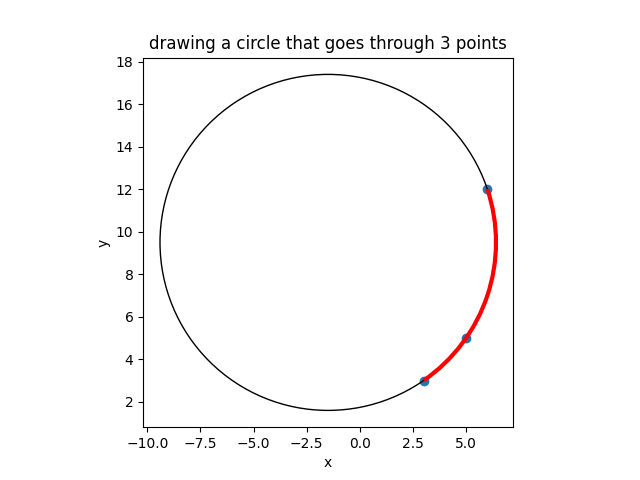
\includegraphics{test}

\begin{center}
Figure 1 - illustration of a circle drawn with matplotlib.patch.Circle
\end{center}


To draw the arc of circle, i used matplotlib.patch.Arc, and basic linear algebra to calculate the right angles delimiting the arc. This is what I explained in the following section.




\subsection{Creating arcs of circle}
Curves aren't full circle, so it's necessary to be able to generate the needed portion of circles. To do so, let's consider the complex plane. In this plane, let assume that \mbox{$z_0 = x_0 + iy_0$} is the center of a circle with a \mbox{$R > 0$} radius. Let assume that \mbox{$z_1$}, \mbox{$z_2$} and \mbox{$z_3$} are points in this circle.  Let assume that \mbox{$\theta_i$} with \mbox{$i \in \left\{1,2,3\right\}$}  are principal complex angles of  \mbox{$z_i$} in the complex affine space centered on the affix \mbox{$z_0$}. Without any loss of generality, let assume that \mbox{$\theta_1 < \theta_2 < \theta_3$}. By using Euler formula, We can get the following equation : 
\[X + iY =  \rho cos(\theta_i) + i\rho sin(\theta_i)\]
with :
\newline
\mbox{$X = x_i - x_0$}
\newline
\mbox{$Y = y_i - y_0$}
\newline
\mbox{$\rho = \sqrt(X^2 + Y^2)$}
\newline
\newline
thus, \mbox{$tan(\theta_i) = Y/X$}
\newline
\newline
therefore, if X > 0 : 

\mbox{$\theta_i = \arctan((y_i - y_0)/(x_i - x_0))$}
\newline
else : 

\mbox{$\theta_i = \arctan((y_i - y_0)/(x_i - x_0)) + \pi$}
\newline
\newline
Now that we have the angles of points, we can use the matplotlib.patches.Arc function to draw the arc of circle, as shown in the previous figure.


\subsection{building a road with no straight lines}
By using the previous method on how to draw arc of circles by using control points in input,  I tried to build my frist attempt of roads. The idea is simple : constructing arc of circles mutually adjacents such that the first control point of one arc is the last control point of the next one. To do so, I needed to generate more than tree control points, so using a mathematical function might be useful in the case. In this case, I used a lambda expression. By constructing such a Python method to display what I just described, I can get the following the result : 

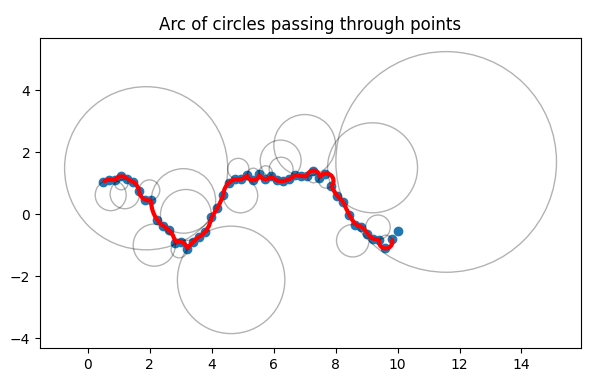
\includegraphics{circleMultiplePoints}
\begin{center}
Figure 2 - representation of a road without any straight lines (circleMultiplePoints(pointsGenerator(0.5,10,50,lambda x : math.cos(x) + math.sin(x)**2,0.2, False))
\end{center}

Unfortunately, this method of drawing roads is unrealistic, since in reality, road contains roughly as much straight lines as turns. Thus, at this point of the project, I had to improve my model.

\section{Road constructors}

In order to create straight lines and curvatures, I came with two approaches. The first one was to create circles, and drawing tangents connecting two consecutive circles. That way, the curvature can easily be obtained by drawing the arc of circle (on the circle) between the two tangent points of a given circle. This is what I called a "global approach", since the road isn't constructed "linearly", but all straight lines first, then curvatures. My second approach was inspired by the idea of building roads "linearly", that is to say in the same order chronologically than a car would ride on the road. In this algorithm, the input is made of an initial point, an initial angle, then a list of angles and a list of distances.

\subsection{Road constructor (first approach) : circles of turns in input}

In this process, circles of turns constitute the input. I define "circle of turn" any circle that has an arc of itself included into the considered road. In other words, a "circle of turn" is an object used to display a curvature of the road. More precisely ans technically, input are radiuses and coordinates of the centers of circles. 

\subsubsection{Tangents as straight sections of roads}

To build straight sections of roads, I proceeded as following. Let's consider two circles, the circle \mbox{$C_1$} defined with a radius \mbox{$R_1$} and centered in \mbox{$L1 = (xL1, yL1)$}, and the circle \mbox{$C_2$} defined with a radius \mbox{$R_2$} and centered in \mbox{$L1 = (xL2, yL2)$}.

\begin{figure}[H]
\centering
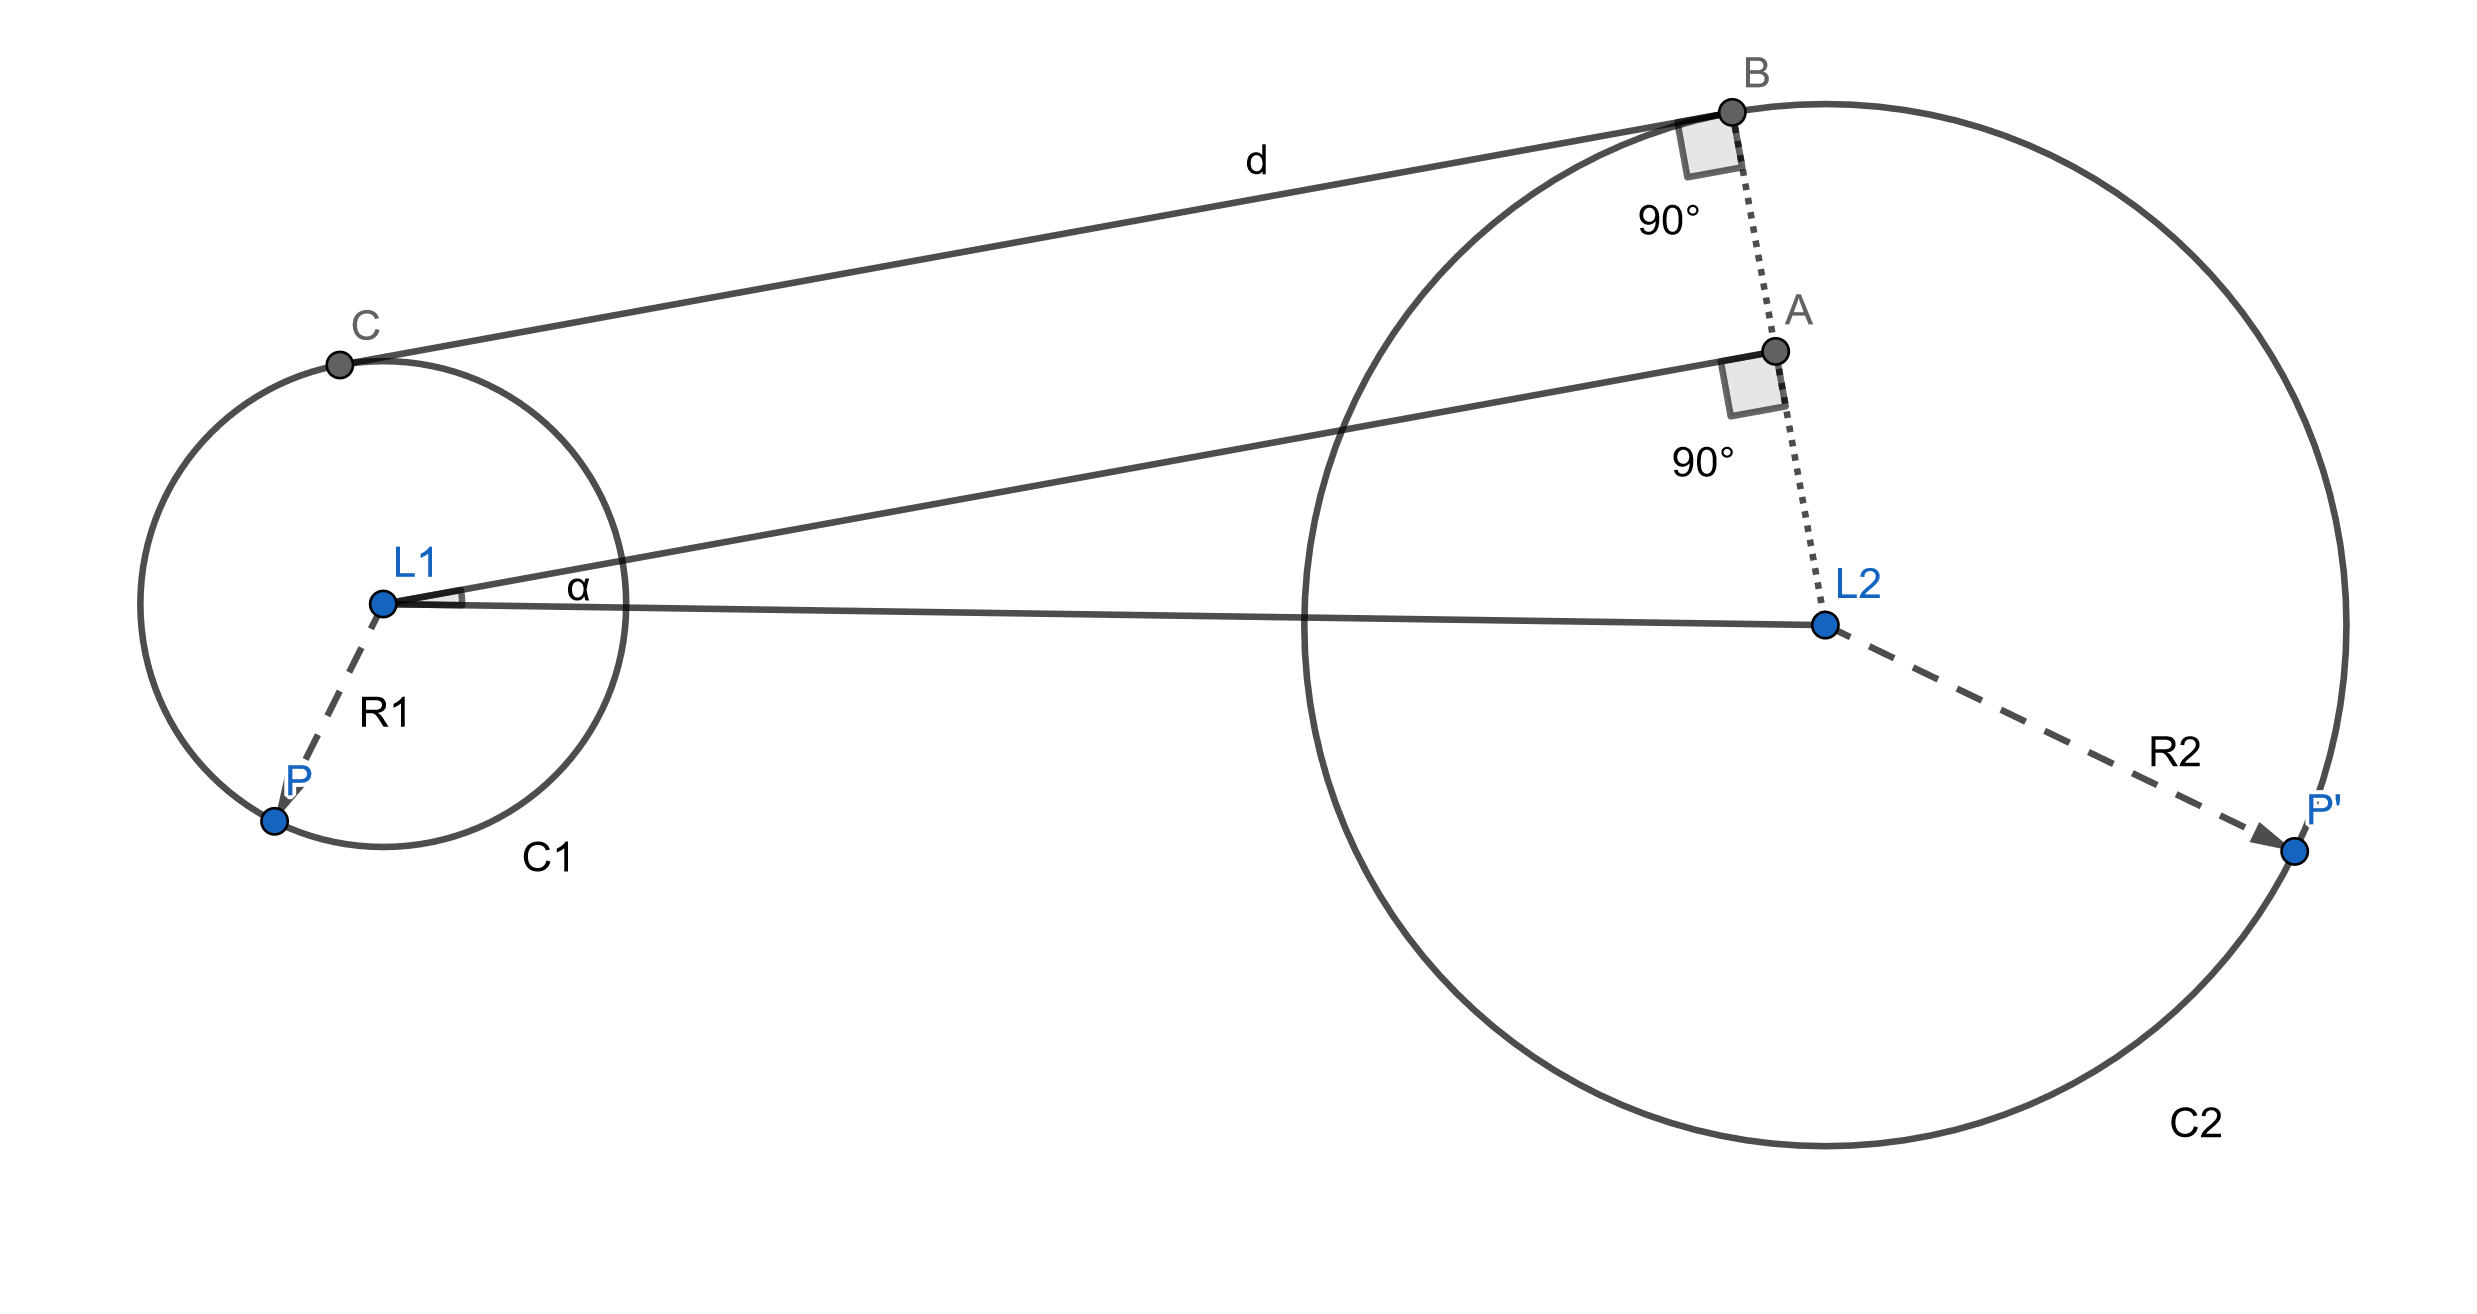
\includegraphics[width=\textwidth]{roadConstructor}
Figure 3 -  geometric representation of notations used for the road constructor, created with Geogebra [5]
\end{figure}

The goal is to build the segment [CB]. For that, we need the coordinates of the point \mbox{$C$} and those of the point \mbox{$B$}. Let's consider \mbox{$O$} the origin of the two dimensional plane. The goal is then to find \mbox{$\overrightarrow{OB}$}. Let's consider \mbox{$\overrightarrow{OB} = \overrightarrow{OL_2} + \overrightarrow{L_2B}$}. Since \mbox{$L_2$} is already known, the vector \mbox{$\overrightarrow{OL_2}$} is already known as well : \mbox{$\overrightarrow{OL_2} = (xL2, yL2)$}. Let's find \mbox{$\overrightarrow{L_2B}$}. \mbox{$\overrightarrow{L_2B} = (R_2 / \lVert \overrightarrow{L_2A} \rVert) \overrightarrow{L_2A}$}. Hence, 

\[ \overrightarrow{OB} = \overrightarrow{OL_2} + \frac{R_2}{R_2 - R_1}\overrightarrow{L_2A}\]
similarly,
\[ \overrightarrow{OC} = \overrightarrow{OL_1} + \frac{R_1}{R_2 - R_1}\overrightarrow{L_2A}\]
The objective is now to get \mbox{$\overrightarrow{L_2A}$}. \mbox{$\overrightarrow{L_2A} = \overrightarrow{OA} - \overrightarrow{OL_2}$}. Besides, \mbox{$\overrightarrow{OA} = \overrightarrow{OL_1} + \overrightarrow{L_1A}$}. Moreover, \mbox{$\overrightarrow{L_1A} = \frac{d}{\lVert \overrightarrow{L_1L_2} \rVert}R_\alpha \overrightarrow{L_1L_2}$} with \mbox{$R_\alpha = \begin{pmatrix} 
cos(\alpha) &  -sin(\alpha)\\ 
sin(\alpha) & cos(\alpha) \\ 
\end{pmatrix}$} and \mbox{$\lVert \overrightarrow{L_1L_2} \rVert = \sqrt{(R_2 - R_1)^2 + d^2}$} and \mbox{$\alpha = arcin(\frac{R_2 - R_1}{\lVert \overrightarrow{L_1L_2} \rVert})$}.Therefore, \mbox{$\overrightarrow{L_2A} = \overrightarrow{OL_1} - \overrightarrow{OL_2} + \frac{d}{\sqrt{(R_2 - R_1)^2 + d^2}}R_\alpha \overrightarrow{L_1L_2}$}. That is to say : 

\[ \overrightarrow{L_2A} = [\frac{d}{\sqrt{(R_2 - R_1)^2 + d^2}}R_\alpha - I] \overrightarrow{L_1L_2} \]
Finally,


\[\overrightarrow{OB} =  \overrightarrow{OL_2} + \frac{R_2}{R_2 - R_1}[\frac{d}{\sqrt{(R_2 - R_1)^2 + d^2}}R_\alpha - I] \overrightarrow{L_1L_2}\]
\[\overrightarrow{OC} =  \overrightarrow{OL_1} + \frac{R_1}{R_2 - R_1}[\frac{d}{\sqrt{(R_2 - R_1)^2 + d^2}}R_\alpha - I] \overrightarrow{L_1L_2}\]

Since B and C are determined, a tangent of \mbox{$C_1$} and \mbox{$C_2$} can be traced.








\subsubsection{Arcs of circle as curve sections of roads}

This version of road constructor is using the same method to building arc of circles described previously in the 1.2 paragraph.

\subsubsection{turning in both direction : inner-outer tangents}

by combining straight lines and curves, I was able to generate this kind of result :

\begin{figure}[H]
\centering
\includegraphics[width=\textwidth]{roadConstructorPlot}
Figure 4 - rendering of the road constructor by calling the roadConstructor() function
\end{figure}

the main problem with this method is that two circles have four tangents together (inner and outer kind of tangents), as I illustrated above with Geogebra, whereas the previous method is always using only one. 

\begin{figure}[H]
\centering
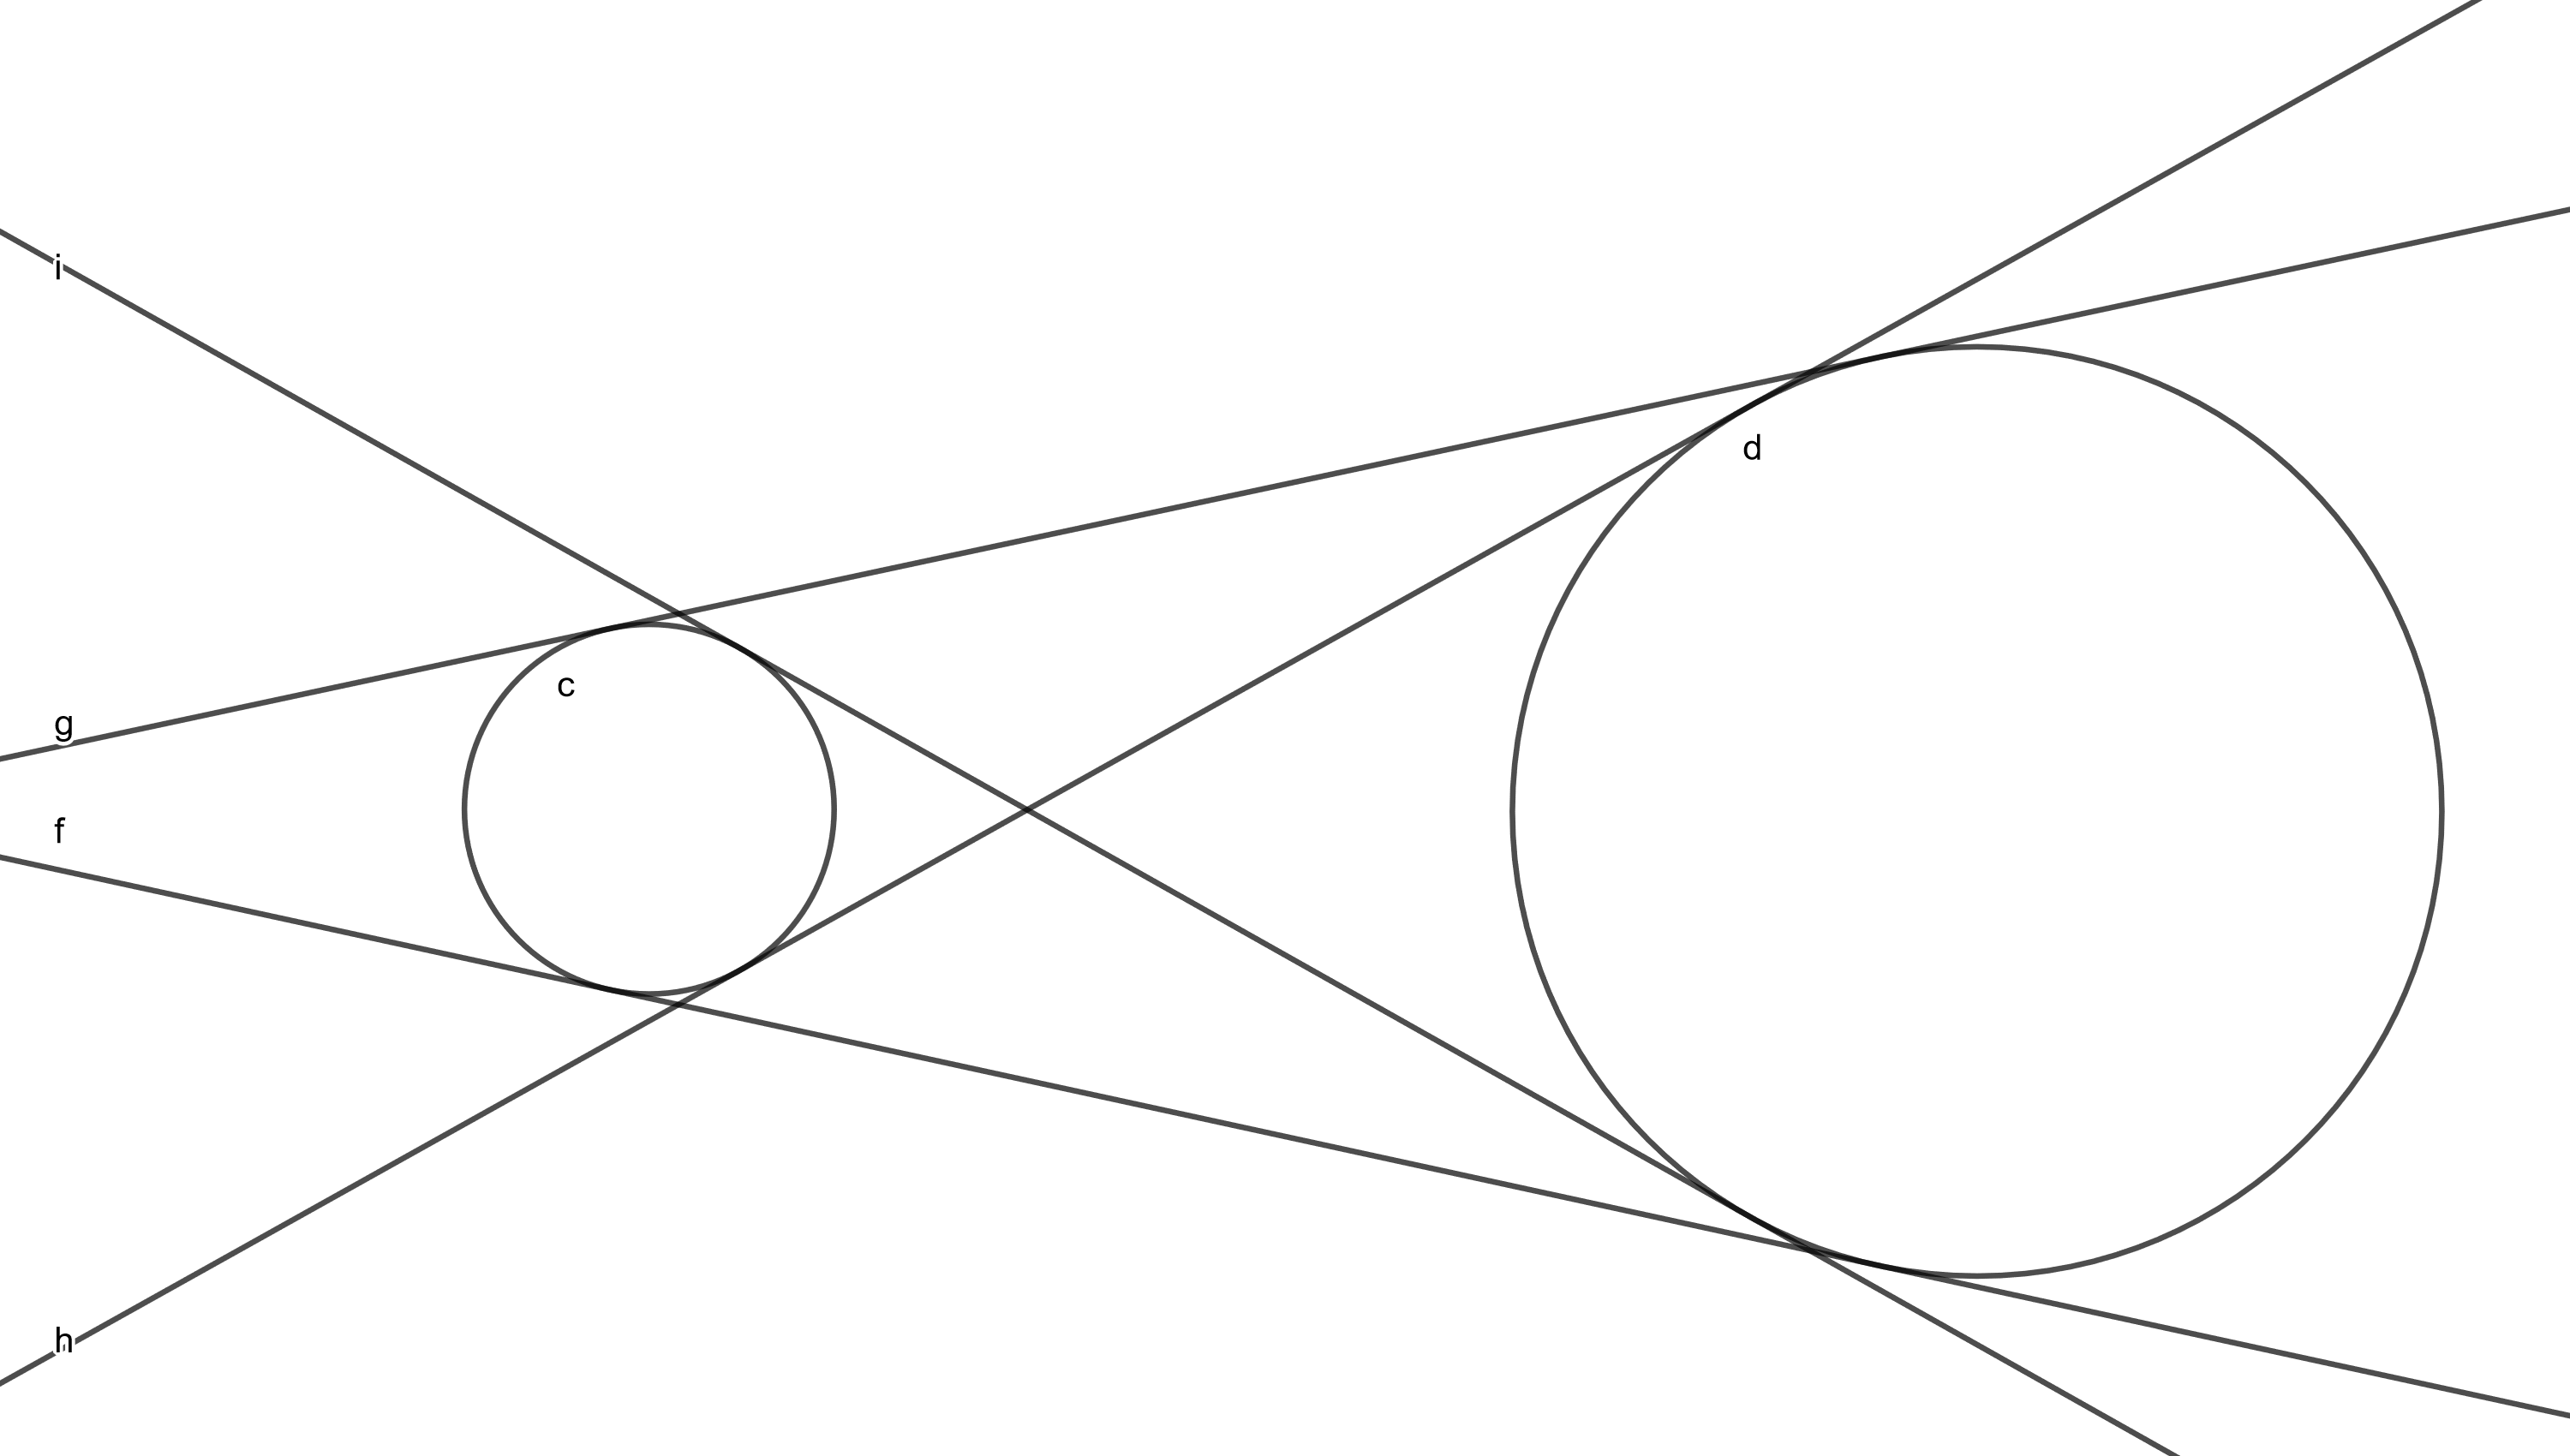
\includegraphics[width=\textwidth]{tangentGeogebra}
Figure 5 - illustration of tangents between two circles
\end{figure}

The consequence of that is that turns are only made in one direction, which is not what we wish for. In order to turn in the other directions, it is necessary to be able to create inner tangents. The prodecure to do so is similar as described in 2.1.1 and 2.1.2. The only different equations are the following :
\[ \lVert \overrightarrow{L_1L_2} \rVert = \sqrt{(R_2 + R_1)^2 + d^2}\]
\[ \overrightarrow{OB} = \overrightarrow{OL_2} + \frac{R_2}{R_2 + R_1}\overrightarrow{L_2A}\]
\[ \overrightarrow{OC} = \overrightarrow{OL_1} - \frac{R_1}{R_2 + R_1}\overrightarrow{L_2A}\]
\[ \alpha = arcin(\frac{R_2 + R_1}{\lVert \overrightarrow{L_1L_2} \rVert})\]

However, this construction done only for a pair of outer-inner tangents (illustratrated in red in this case) :

\begin{figure}[H]
\centering
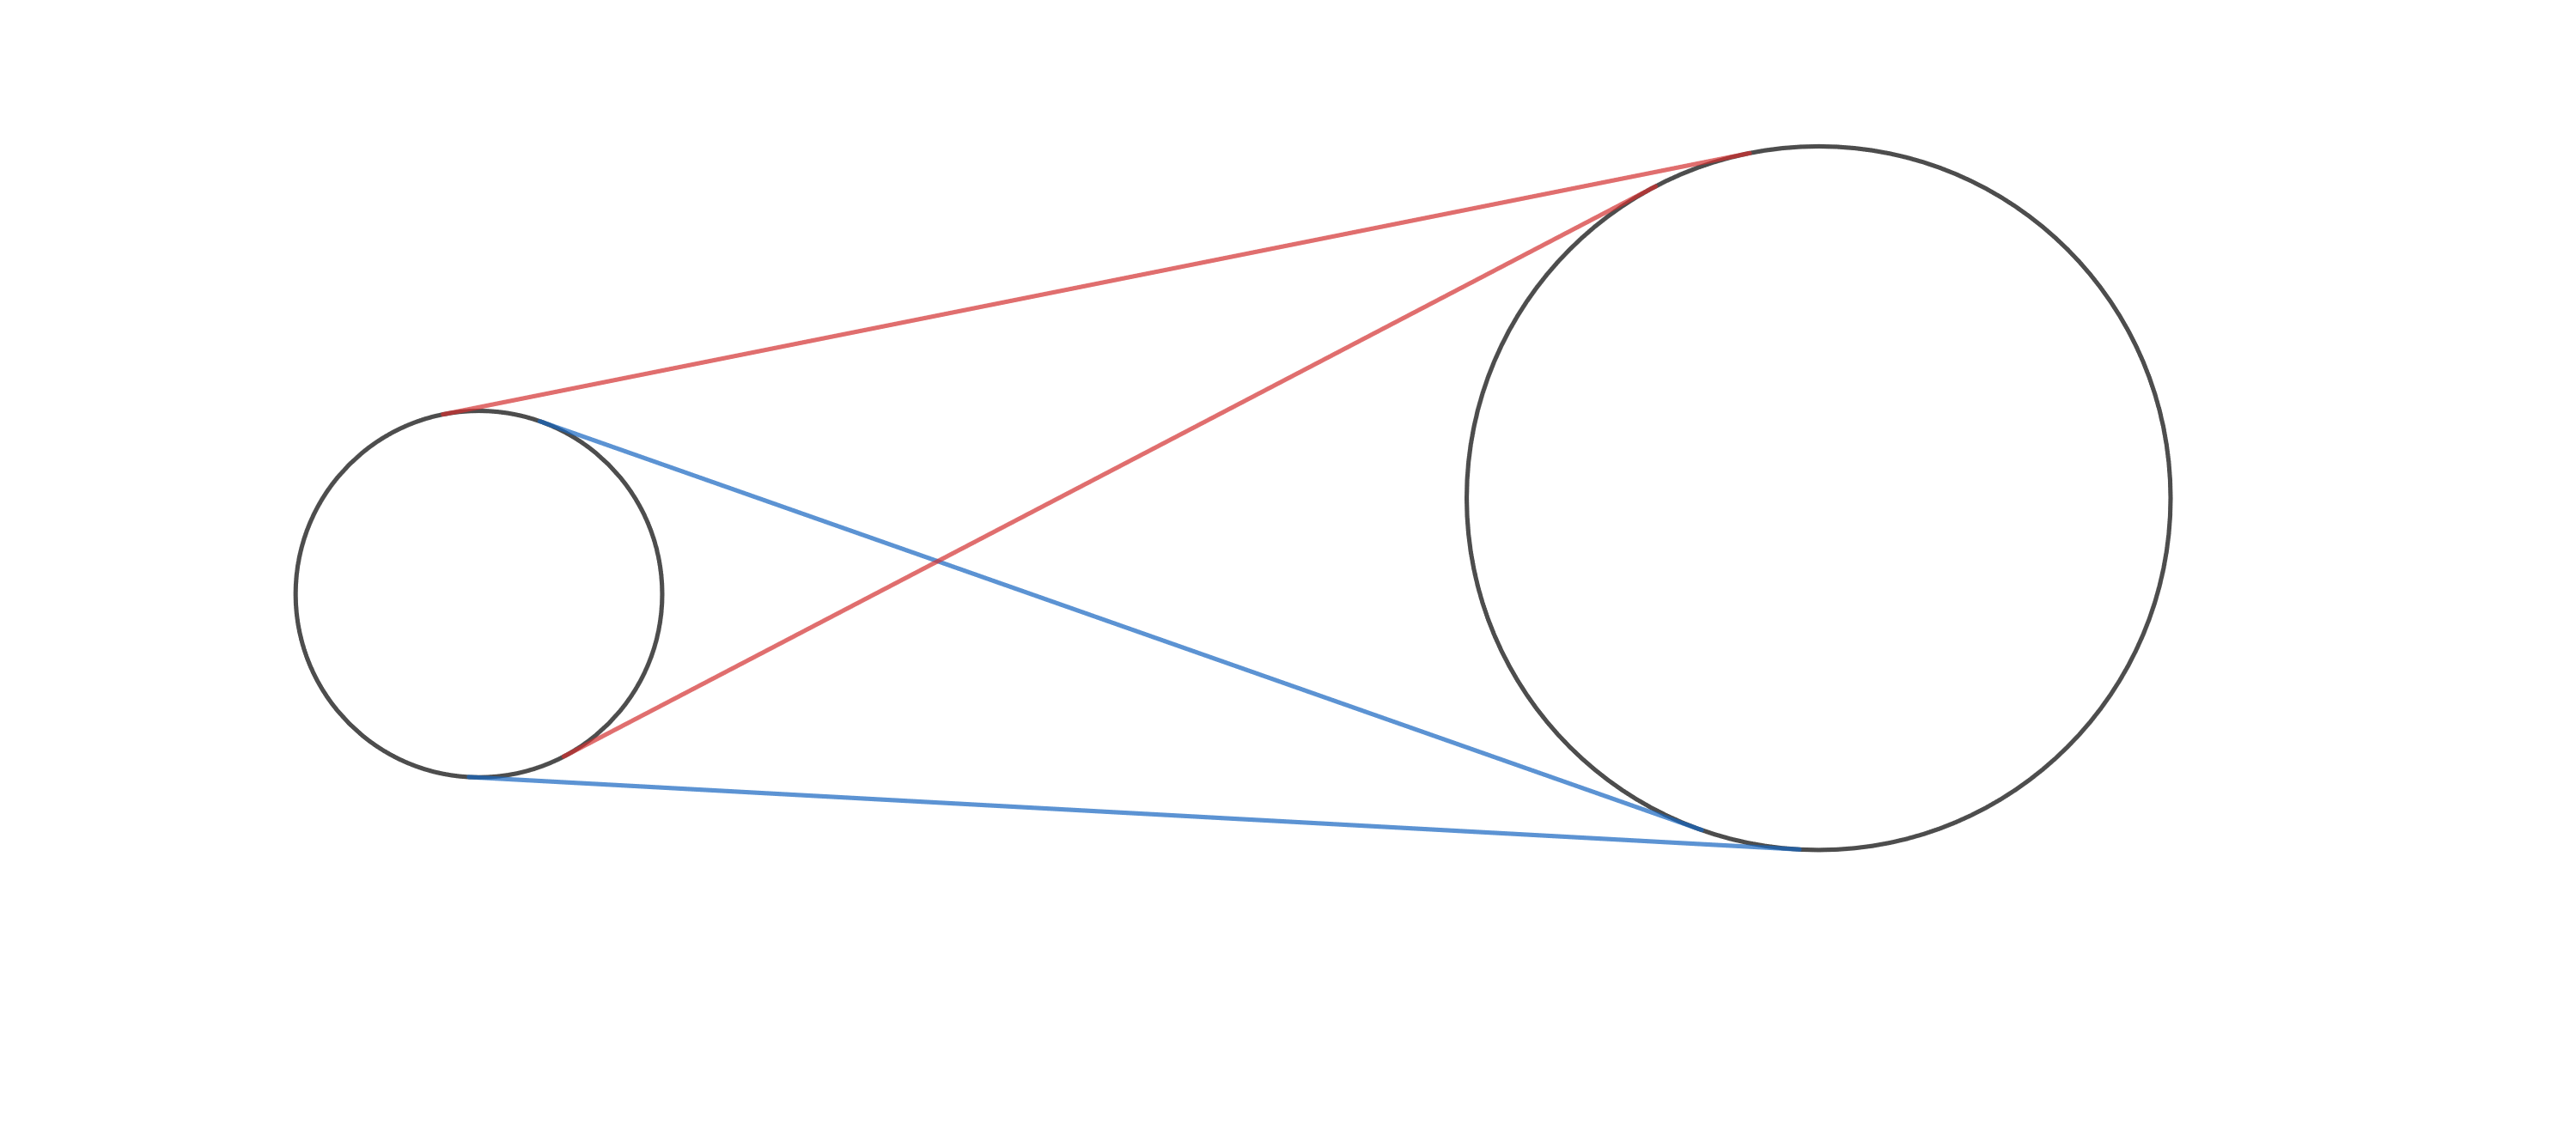
\includegraphics[width=\textwidth]{tangentsRoad}
Figure 5.1 - illustration of two pairs of inner-outer tangents
\end{figure}

To generate the blue pair, the only thing to do is to permut the sign of \mbox{$\alpha$}. That way, I was able to generate this kind of result :

\begin{figure}[H]
\centering
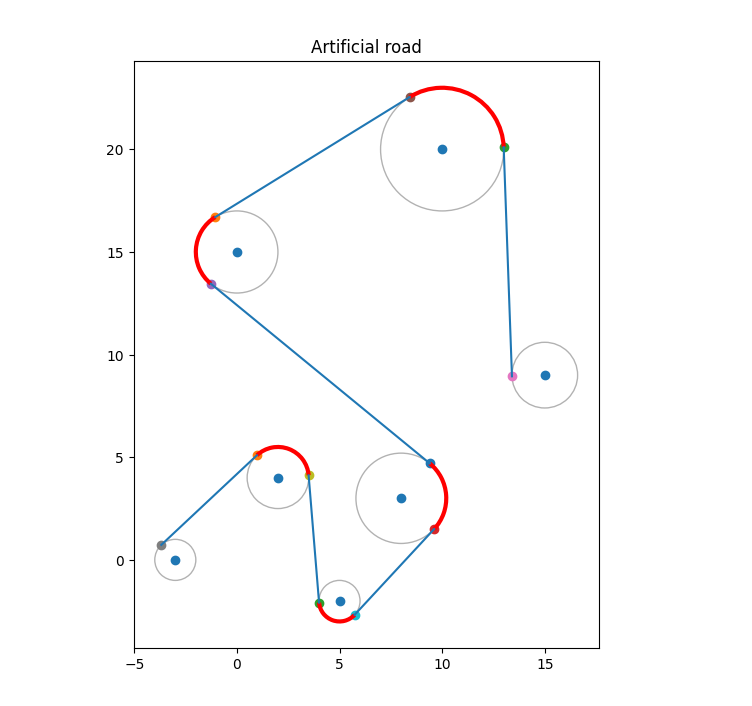
\includegraphics[width=\textwidth]{roadConstructorFinal}
Figure 5.2 - illustration of a road using all four combinations of turns possible, that is to say "clockwise anti-clockwise", "clockwise clockwise", anti-clockwise anti-clockwise" and "anti-clockwise clockwise" turns. Function called : roadConstructor(True, [1,-1.5,1,-2.2,2,-3,1.6], [-3,2,5,8,0,10,15], [0,4,-2,3,15,20,9], [1,-1,-1,1,1,-1]).
\end{figure}




This method does not fit very well if I want to use it by using real sampled data in input. In this method, input are circles, not sampled points of a road, which would make the inverse-engineering part of the project nearly impossible. In addition, I couln't be able to find a way to automatically determine the sign of  \mbox{$\alpha$} in order to choose the correct pair of inner-outer tangents, so if the user wants to generate a road, he had to specify it manually among the argument of the roadConstructor() function. Those reasons contributed to motivate me to seek for another method to generate roads.


\subsection{road constructor (second approach) : angles and lengths as inputs }

In this second approach, roads are constructed progressively. Initially, the road starts with a starting points, a direction, and a length which determines the first line of the road. Then, an alternation of curves and straight lines are created and determined by a set of angles (which describes the curvatures of turns) and a set of length (which describes the length of straight lines). In this algorithm, radiuses of circles of turns are all the same, contrary to the previous road constructor approach.

\subsubsection{from the starting point to the first turn}

Let's call \mbox{$P_1{'}$} the starting point of the road, \mbox{$l_1$} the length of the first straight section, \mbox{$\alpha_1$} the angle determining the direction of the first straight section,  \mbox{$P_2$} the first point of the turn, \mbox{$P_2{'}$} the last one, \mbox{$\alpha_2$} the angle determining the first turn section, and finally \mbox{$R$} the radius of turns.

\begin{figure}[H]
\centering
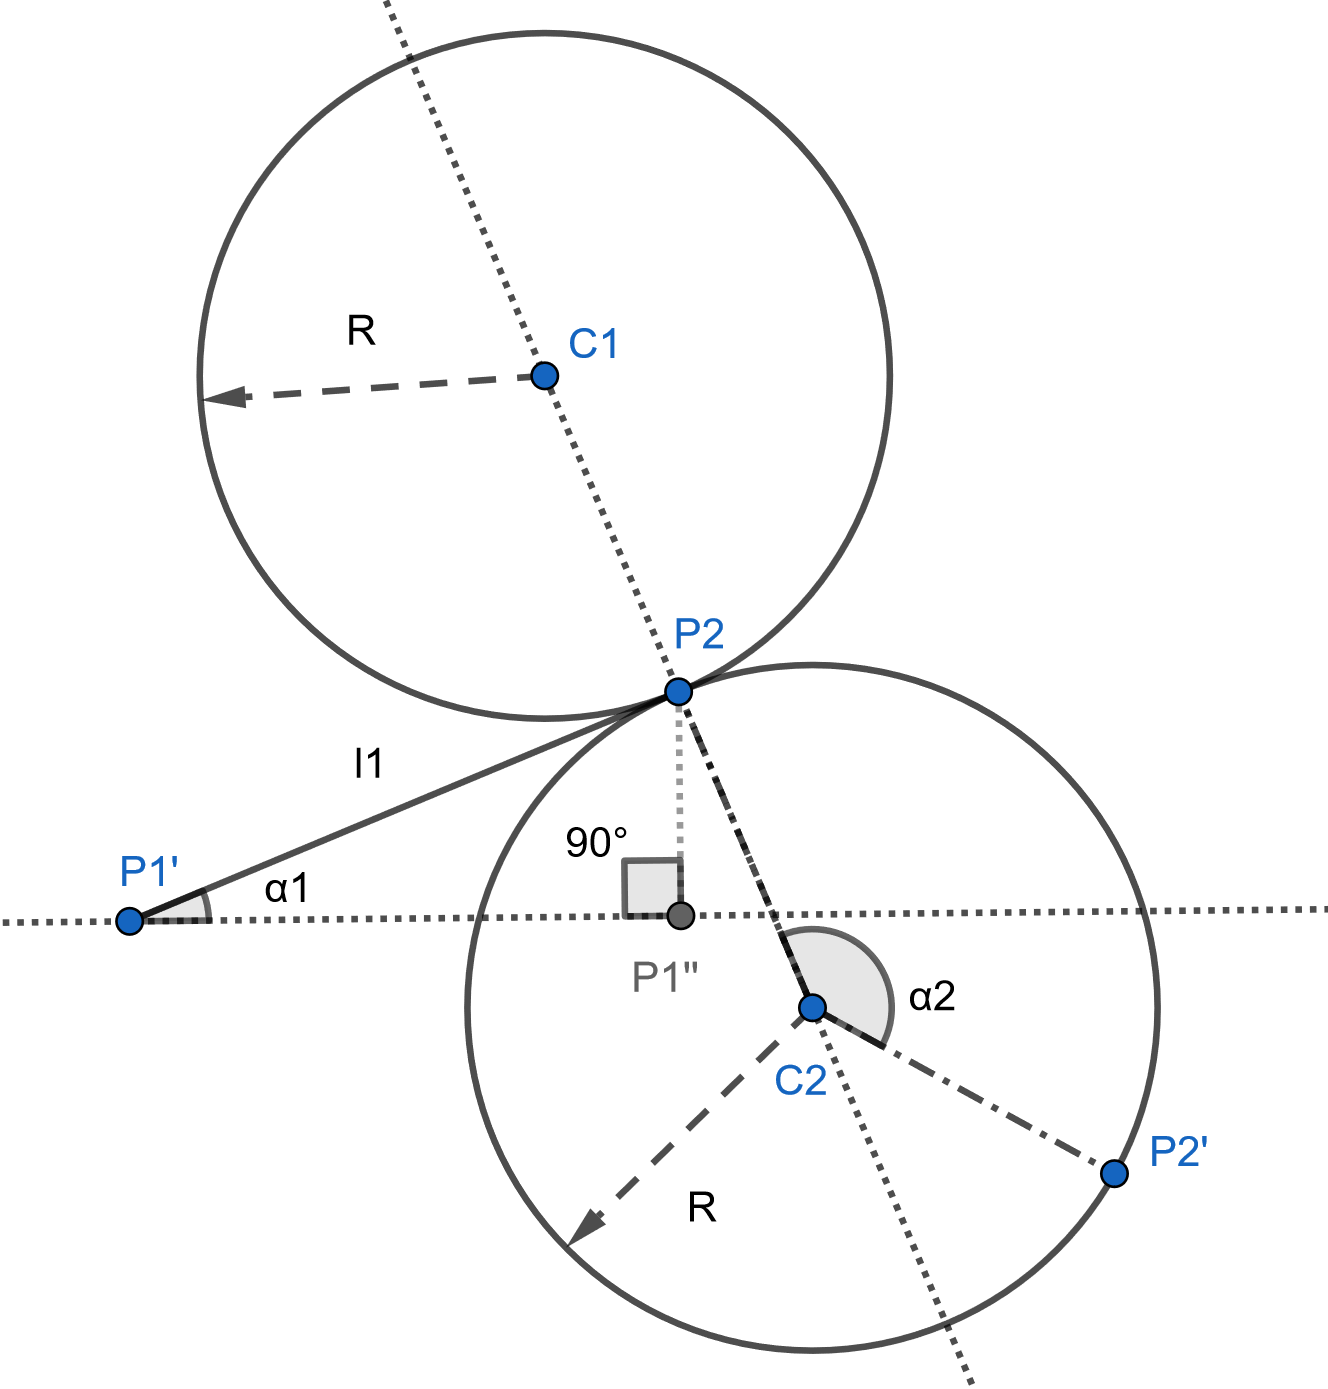
\includegraphics[width=\textwidth]{roadConstructor2Geogebra}
Figure 6 - Geogebra illustration of notations for the first turn
\end{figure}

the goal is to be able to generate \mbox{$P_2$} and \mbox{$P_2{'}$} with \mbox{$P_1{'}, \alpha_1, l_1$} in input. First, let's focus on \mbox{$P_2$} \mbox{$\overrightarrow{OP_2} = \overrightarrow{OP_1{'}} + \overrightarrow{P_1{'}P_2}$}. Besides,  \mbox{$\overrightarrow{P_1{'}P_2} = \frac{l_1}{\lVert \overrightarrow{P_1{'}P_1{''}} \rVert} R_(\alpha_1) \overrightarrow{P_1{'}P_1{''}}$}
with \mbox{$R_(\alpha_1) = \begin{pmatrix} 
cos(\alpha_1) &  -sin(\alpha_1)\\ 
sin(\alpha_1) & cos(\alpha_1) \\ 
\end{pmatrix}$}. 
\newline
Moreover, \mbox{$\lVert \overrightarrow{P_1{'}P_1{''}} \rVert = \sqrt{l_1^2 - (sin(\alpha_1)l_1)^2}$}. Therefore,

\[ \overrightarrow{OP_2} =  \overrightarrow{OP_1{'}} + \frac{l_1}{\sqrt{l_1^2 - (sin(\alpha_1)l_1)^2}} R_(\alpha_1) 
\begin{pmatrix}
\mbox{$xP_1{'} + \sqrt{l_1^2 - (sin(\alpha_1)l_1)^2}$} \\
\mbox{$yP_1{'}$}
\end{pmatrix}	
\]

Let's find \mbox{$P_2{'}$}. Suppose that \mbox{$\alpha_2 \in [-\pi, \pi]$}. Let assume that \mbox{$\alpha_2 < 0$} (this case is illustrated in figure 6).
\mbox{$\overrightarrow{C_2P_2{'}} = R_(\alpha_2) \overrightarrow{C_2P_2}$} with \mbox{$R_(\alpha_2) = \begin{pmatrix} 
cos(\alpha_2) &  -sin(\alpha_2)\\ 
sin(\alpha_2) & cos(\alpha_2) \\ 
\end{pmatrix}$}. 
\newline
Moreover, \mbox{$\overrightarrow{C_2P_2} = - \frac{R}{l_1} R_(-\pi/2)\overrightarrow{P_1{'}P_2}$} with
\mbox{$R_(- \pi/2) = \begin{pmatrix} 
0 &  1\\ 
-1 & 0 \\ 
\end{pmatrix}$}.
\newline
Moreover, \mbox{$\overrightarrow{OP_2{'}} = \overrightarrow{OP_2} + \overrightarrow{P_2C_2} + \overrightarrow{C_2P_2{'}}$}
\newline
Therefore,
 
\[\overrightarrow{OP_2{'}} = \overrightarrow{OP_1{'}} + \frac{l_1}{\sqrt{l_1^2 - (sin(\alpha_1)l_1)^2}} R_(\alpha_1) 
\begin{pmatrix}
\mbox{$xP_1{'} + \sqrt{l_1^2 - (sin(\alpha_1)l_1)^2}$} \\
\mbox{$yP_1{'}$}
\end{pmatrix} + \frac{R}{l_1} R_(-\pi/2)[Id - R_(\alpha_2)]\overrightarrow{P_1{'}P_2}\]

if \mbox{$\alpha_2 >= 0$}, the procedure is the same, but \mbox{$C_2$} has to be replaced by \mbox{$C_1$}.




\subsubsection{from the first turn to the next one, result}

Suppose that we successfully generated the first part of the road : the straight line and the turn. In order to generate the following part, we can reuse what was already done. Indeed, One can consider that the "new" initiate point is \mbox{$P_2{'}$} and the "new" initiate length is \mbox{$l_2$}. I proceeded that way until every initial ressources (length and angles) in the input are depleted. That way, I was able to generate the following plot :


\begin{figure}[H]
\centering
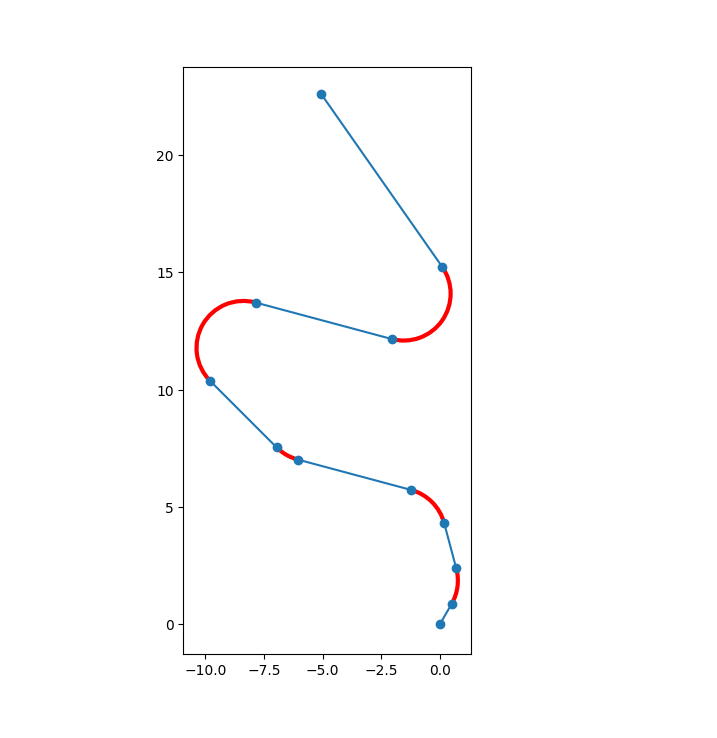
\includegraphics[width=\textwidth]{roadConstructor2}
Figure 7 - rendering of the road constructor (version 2) by calling the roadConstructor2() function
\end{figure}


As we can see,  by construction, turn to the left and to the right are possible. However, due to the limitation of my models, U-turns aren't possible since \mbox{$\alpha_2 \in [-\pi, \pi]$}. Consequently, without extending and generalizing this algorithm, loops aren't possible. This approach is better is my opinion, because it's easier to predict where the road will be generated. Furthermore, It's also easier to add controlled modification by slightly changing a length or and angle for example. Thus, this approach gives more control and freedom to the user.

 


\section{Retro-engineering of roads}

Let's assume that we may want to recreate a road based on sampled data. Such sampled data are basically ordered points spacially distributed on a two dimensional plane. Before trying to build an algorithm that can help me to "retro-engineer" a road, I deem necessary to work in the first place on artificial sampled data. To do so, it is necessary to be able to generate such sampled data points.

\subsection{sampling roads}

Let's take for instance the following road :

\begin{figure}[H]
\centering
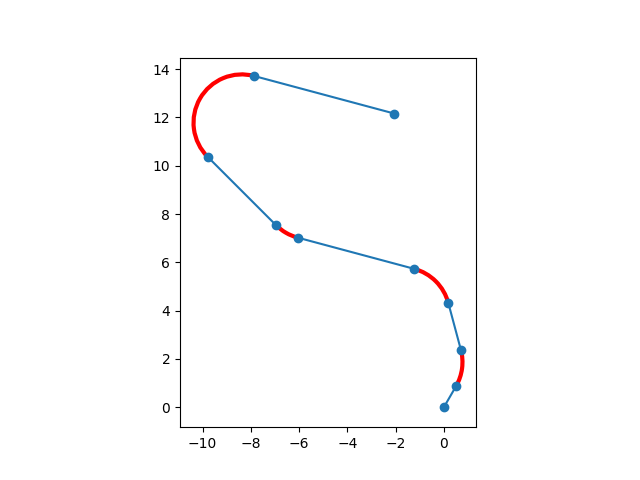
\includegraphics[width=\textwidth]{sampledRoadRoad}
Figure 8 - rendering of the road constructor (version 2) by calling the roadConstructor2() function
\end{figure}

This plot has been generated by calling roadConstructor2([0,0],2,math.pi/3,[np.pi/4, np.pi/3, -np.pi/6, -5*np.pi/6],[2,5,4,6],2,False). We are looking how to sample the road. The sampleRoad() function is doing so, by sampling straight lines and turns. The algorithm is sorting points in order to preserve the original order of the road.  After the sampling process, we get this result : 


\begin{figure}[H]
\centering
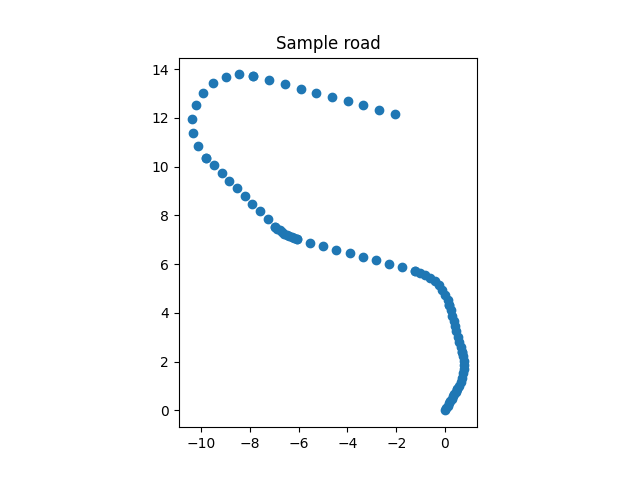
\includegraphics[width=\textwidth]{sampledRoadPoints}
Figure 9 - rendering of the sampled road illustrated in figure 8, using the sampleRoad() function
\end{figure}
Note that the density of sample points is not uniform. Indeed, for each road section (line or turn), a given number of points on the road will be sampled. Thus, the shorter the section, the denser are the points. This plot has been generated by calling 
\newline
sampleRoad(roadConstructor2([0,0],2,math.pi/3,[np.pi/4, np.pi/3, -np.pi/6, -5*np.pi/6],[2,5,4,6],2,False)).
\newline
\newline
In order to re-build the road with sampled data in input, it is necessary to detect where straight and turn sections of the road can possibly be.

\subsection{detection of straight lines : linear regression method}

For the sake of trying to detect straight section, I wrote the regressionLines() method. The idea to do so is the following. First, the algorithm takes the very first amount of sampled points of the roads, starting from the beginning. This number is determined by the argument thresholdEnd. Then, a linear regression is done through those points. If the regression is good enough (that is to say, if the r-value of the fitting line is above a given limit r value called limrvalue), then the algorithm can deduce that there those points are aligned. The closer the square of the r-value is to 1, the better is the approximation. However, at that moment, it's not possible to infer how long the straight line is : the only fact inferred is that the road is likely to contains at least the very first points as a straight line. Thus, in order to check if this line is longer or not, the algorithm takes the next point and do the previous procedure : creation of a fitting line but with one additional point. This goes until either all points are depleted and used by the algorithm, either the r-value is not good enough. In the case where the r-value is not good enough, if the number of points selected is great enough (greater than thresholdCurve), then the algorithm infers that points are likely to be aligned. If it's not the case (number of points selected smaller than thresholdCurve),  the sequence of points is too short to be a straight line, hence it can be deduced that it's likely to be a turn. The same reasoning is applied when all points are depleted and used by the program. Once an estimation by the function is made regarding the sequence of points (straight line or curve), the same algorithm is applied by considering not the first point of the sampled roads, but the last one of the previous iteration. This goes on until the last sample of the dataset.
\newline
 \newline
 A particular problem that I noticed is the detection of false straight section of roads in turns. However, this problem is purely due to the choice of parameters, but still remains an issue since parameters are set manually in an absolute manner : they are not automatically related to the sample. For instance, with the sample road illustated in figure 9, I got the following result :


\begin{figure}[H]
\centering
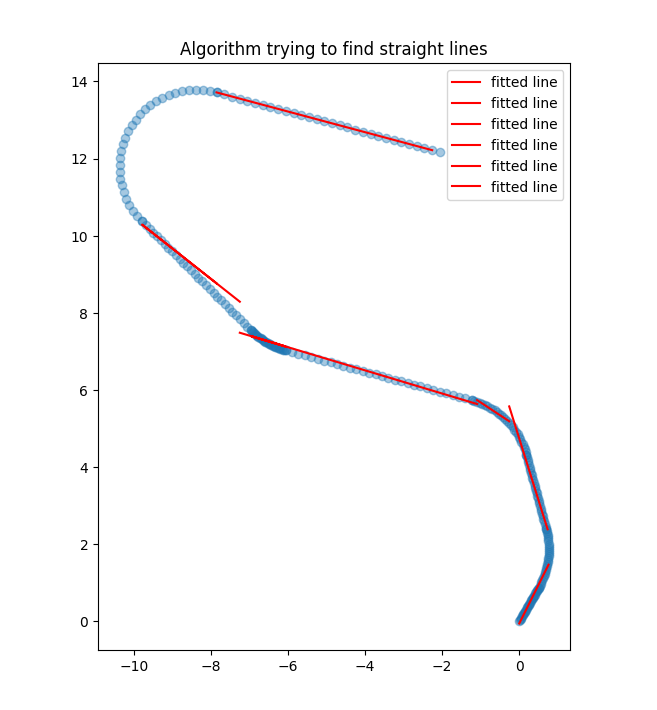
\includegraphics[width=\textwidth]{regressionLine}
Figure 10 - rendering of a sampled road, with fitted lines that predict where straight section of the road can possibly be
\end{figure}
To get this rendering, regressionLines(sampleRoad(roadConstructor2([0,0],2,math.pi/3,[np.pi/4, np.pi/3, -np.pi/6, -5*np.pi/6],[2,5,4,6],2,False)),3,0.95,15) was called. Note that the quality of the result highly depends of the choice of the parameters that are the arguments of the regressionLines() function... which depends of the sample! In other words, in order to have a decent quality for the straight line detection, parameters depend of the sample since parameters are set manually and "absolutely". This represents a flaw of the algorithm since it would make hard to apply this function to a broader variety of sampled road. Furthermore, the number of sampled roads that can provide relatively good results for the regressionLines method is narrowed by the fact that a decent amount of samples are needed to preserve the quality of the approximation of fitted lines.

\subsection{detection of turns : clustering of curvatures}

One idea that I exploited to find the curvature of a road based on his "sampled form" is to proceed as the following. The idea is to use the circleMultiplePoints() function to the sample points in order to display the points and to draw arc of circles going through them, three by three. Then, for each curvature (arc of circle) get the curvature of the turn (which is the opposite of the radius of the circle that was used to draw the arc of circle) and plot the result into a graph as following : 


\begin{figure}[H]
\centering
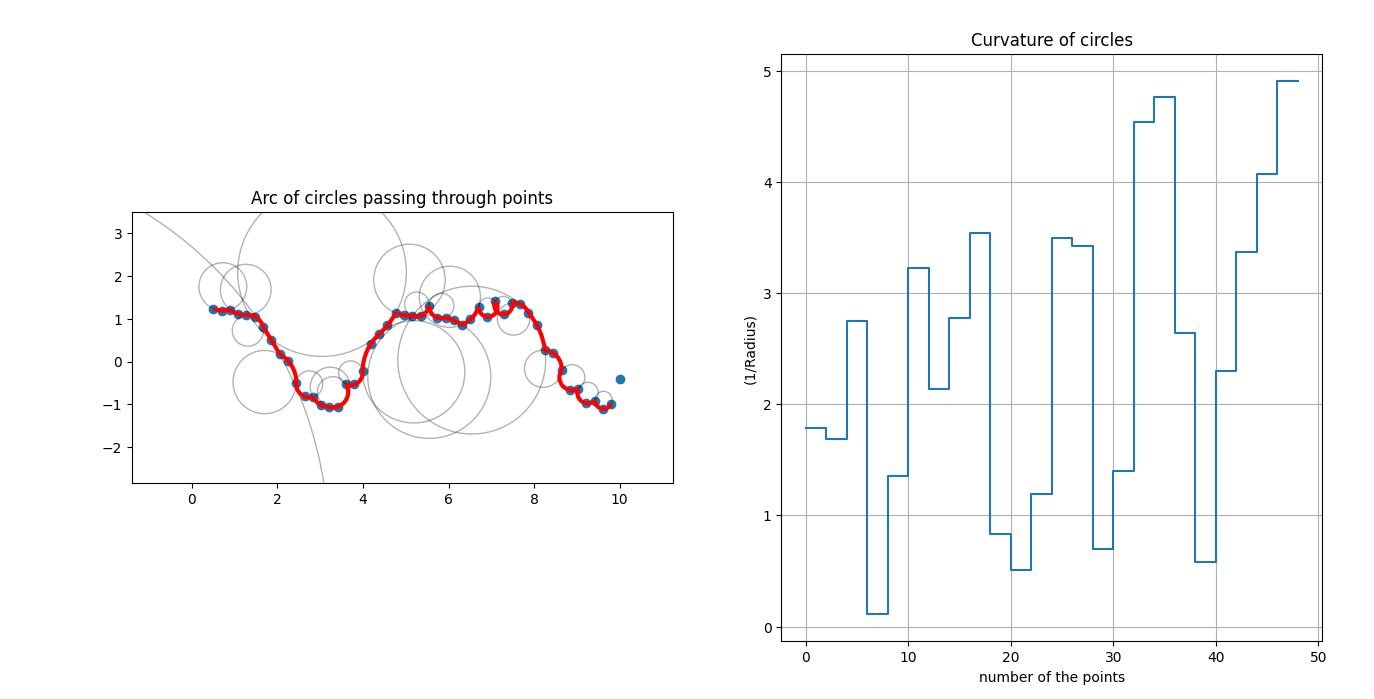
\includegraphics[width=\textwidth]{curvatures}
Figure 11 - rendering of a sampled road with circles going through them three, and the plot of curvature associated
\end{figure}

The plot has been generated by calling circleMultiplePoints(pointsGenerator(0.5,10,50,lambda x : math.cos(x) + math.sin(x)**2,0.2, False)), where pointsGenerator() is a function that, based on a function, returns sampled points of it, but with a little bit a noise (depending of the second argument of the function).
The idea was to cluster curvatures that are "relatively close" to each other in terms of value, then to make the average for each cluster. Afterwards, for each cluster, create an arc of circle whose curvature is the curvature associated with the cluster (which is the average of curvatures of curves clustered). This part of the inverse-engineering process has not been implemented yet in the scope of this coursework.






 %Conclusions section
\sectionWithoutNumber{\keyWordConclusions}{conclu}


Two approaches to build roads have been handled this coursework. the first one allows the user to generate roads with circles in input. The sign of radiuses determines the orientation of turns, and the algorithm is such that all combinaison of turns are possible (included overlapping roads). However, the user has to specifiy manually some additionnal residual necessary information to draw straight portions (to choose which pair of inner-outer tangent to consider) because I coulndn't find a way to automate it. This method of building roads is convenient to modify already generated roads by the latter method, but not so much to actually generating it. The second approach is using directions and lengths as input. This version is functional and turns in both direction are possible. This approach is more local than the previous one and gives more control for the user : it's easier to create a road since the building process is chronologically in the same order as the travel order. In other words, the process is more natural.
\newline
A potential feature that could be added is the data translation from a road built by the second approach to the same road but build by the first approach. That would make both approaches complementary, since roadConstructor2() is more convenient to generate roads and rodConstructor1() to modify them.
Then, I tried to implement a inverse-engineering protocol whose goal was to detect "straight and curve portions of road" among sampled data. My hope was to be able to generate a road akin to the road that have been sampled. "the straight detector" gives very approximate results and sampled data have to be really good and full. The "curve detector" hasn't been implemented.
\newline
During this project, I used Python, which allows me to consolidate my knowledge in that language. I feel better at coding my ideas when it comes to linear algebra. I liked working in this project, even though time was sometimes short. Buvo malonu.


%ateities darbų gairės, planas/next steps of the work
\sectionWithoutNumber{Roadmap and future work}{future}{


One feature missing is the detection of curvatures within a sampled road in the inverse-engineering program. It's a necessary feature, but quite complex and unfortunately I didn't have time to deal properly with it. The inverse-engineering part has been tested on artificial sampled road, in good conditions. It would be nice to test it on real world data. Furthermore, turns can be modeled by other things than circular arc. Using Bézier's curve might produce better modelization. Using clothoïds might be even better. Circular spline might be a great possibility to connect straight portion of roads [3].
}

 %file literatureSources.bib
\referenceSources{literatureSources}



%% this part is optional
\newpage
\begin{appendices}
\section{Bibliography}
\label{app:a}
[1] : PINAVIA, two-level road junction (booklet)
\newline
[2] :  Stephen R. Schmitt. Center and Radius of a Circle from Three Points (2005),.  \url{https://web.archive.org/web/20161011113446/http://www.abecedarical.com/zenosamples/zs_circle3pts.html}
\newline
[3] : Xinghua Song, Martin Aigner, Falai Chen, Bert Jüttler. Circular spline fitting using an evolution process (2009). \url{https://doi.org/10.1016/j.cam.2009.03.002}
\newline
[4] : Matplotlib documentation. \url{https://matplotlib.org/stable/index.html}
\newline
[5] : Geogebra documentation. \url{https://wiki.geogebra.org/en/Manual}
 
\end{appendices}
\end{document}
